\subsubsection*{Inicialización de la GDT}

Inicializamos la Tabla de Descriptores Globales con entradas para segmentos de código de nivel 0 y 3, otras para segmentos de datos de nivel 0 y 3, una para un segmento que describe el área de la pantalla de video, y la entrada correspondiente al segmento donde se guardará la tss de la tarea inicial. (Las entradas de gdt para las tss de las demás tareas son completadas al inicializarlas, como se explica en la sección correspondiente al Ejercicio 6).

\par Se utiliza desde el índice 8 por restricciones del trabajo práctico.
Los segmentos de datos y códigos están organizados de tal forma que se superpongan direccionando los primeros 500MB de memoria (Sistema FLAT), utilizando bloques de 4K al setear el bit de granularidad en 1.
\par Los demás atributos fueron seteados de la siguiente manera:
\par \textbf{\emph{Base y Límite: } }Como mencionamos anteriormente, los segmentos de código y datos están superpuestos. Comienzan en la dirección base 0x00000000, y el valor del límite 0x1F3FF corresponde la cantidad de bloques-1. Es decir, para cubrir 500MB se necesitan 128.000 bloques de 4K. El offset del último bloque es 127.999 (0x1F3FF en hexa).
Con respecto al segmento de video, éste ocupa en memoria desde la posición 0xB8000 hasta la 0xC0000, es decir 32K de memoria, cuyo máximo offset o límite es el correspondiente al último byte (7999 = 0x7FFF).
Para las tss, el límite es 0x68, pues miden 104 bytes cada una. Como base de la tarea inicial, seteamos la dirección 0x0000. ???????
\par \emph{\textbf{Tipo: }} El tipo para los segmentos de código es 0x0A (executable, readable), mientras que para los de datos y video es 0x02 (readable, writable).
\par \emph{\textbf{Sistema: }} El bit de system está seteado en 1 salvo en los segmentos correspondientes a las tss de las tareas, donde está activo bajo en 0 pues son potestad exclusiva del sistema operativo.
\par \emph{\textbf{DPL: }} Los segmentos de datos y código de nivel 0 tienen DPL en 0x00, al igual que los segmentos de sistema y el de video, mientras que los de código y datos nivel 3 tienen DPL en 0x03.
\par \emph{\textbf{Granularidad: }} El bit de G está activo sólo en los segmentos de datos y código ya que es necesario bloques de 4K para abarcar los 500MB.
\par \emph{\textbf{P, L, D/B, AVL: } }Seteados en 1, 0, 1 y 0 respectivamente para todas las entradas.
\newline

\subsubsection*{Pasaje a Modo Protegido}

\par Para pasar a modo protegido, completamos y cargamos la GDT usando la instrucción lgdt, que toma el descriptor de la GDT con el tamaño y la dirección de la misma, habilitamos A20 para habilitar el acceso a direcciones superiores a los 2$^{20}$ bits, seteamos el bit de PE del registro CR0, y saltamos a 0x40:modoprotegido donde el 0x40 corresponde al Indice del segmento de código de nivel 0 (índice 8 en la gdt), corrido 3 ceros (estos ceros son los del TI y RPL).

\begin{lstlisting} [caption={Pasaje a modo protegido},label=modoproteg]
    ; Habilitar A20
    call habilitar_A20  
   
    ; Cargar la GDT
	lgdt [GDT_DESC]      ; cargo la estructura que esta en gdt.c

    ; Setear el bit PE del registro CR0
    mov eax, cr0
	or eax, 1
	mov cr0, eax

    ; Saltar a modo protegido
	jmp 0x40:modoprotegido
\end{lstlisting}


\par Una vez trabajando en modo protegido, procedemos a establecer los selectores de segmentos de datos de nivel 0 (indice 9 en la gdt, corrido tres ceros correspondientes a los bits de TI y RPL), y el selector de segmento de video en fs (indice 12 en la gdt). Luego establecemos la base de la pila en la dirección 0x27000.


\begin{lstlisting} [caption={Pasaje a modo protegido},label=modoproteg2]
    modoprotegido:
    ;Establecer selectores de segmentos
    xor eax, eax
	mov ax,  1001000b
	mov ds, ax
	mov es, ax
	mov gs, ax
	mov ss, ax
    	mov ax, 1100000b
    mov fs, ax

    ; Establecer la base de la pila
	mov ebp, 0x27000
	mov esp, 0x27000
\end{lstlisting}

\subsubsection*{Inicialización de la Pantalla}

\par Para inicializar la pantalla llamamos a la función de screen.h \texttt{screen_inicializar}, que se encarga de pintar la pantalla con el mapa, las barras para los jugadores, e inicializar los slots vacios y puntos en 0 de cada jugador, utilizando las funciones \texttt{screen_pintar_rect} para pintar un rectangulo de color, \texttt{print_dec} para imprimir los puntos, y \texttt{screen_pintar} para imprimir caracteres.

\begin{figure}[ht!]
\centering
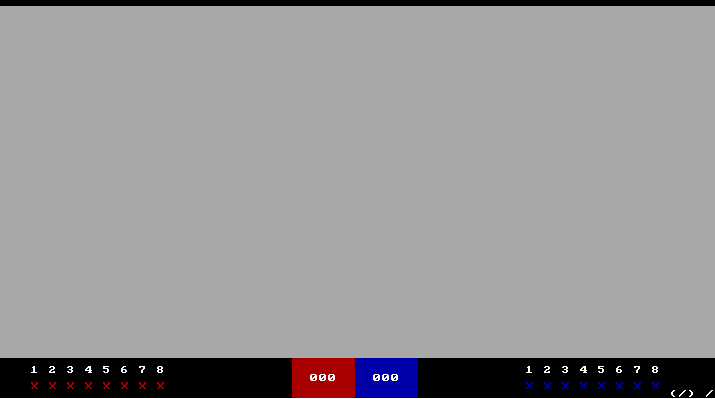
\includegraphics[width=120mm]{imagenes/pantalla.png}
\caption{Pantalla Inicial.}
\end{figure}